%-----------------------------------------------------------------------------%
\chapter{\babTiga}
%-----------------------------------------------------------------------------%
%-----------------------------------------------------------------------------%
\section{Tahapan Penelitian}
%-----------------------------------------------------------------------------%
Secara garis besar, tahapan penelitian yang hendak dilaksanakan dalam penelitian ini terdiri dari beberapa tahapan utama yaitu studi literatur, perancangan metode, pengumpulan data, implementasi program, evaluasi dan analisis hasil. Bagan tahapan penelitian dapat dilihat pada \ref{fig:metodologi_penelitian} berikut:

\begin{figure}[htp]
	\centering
	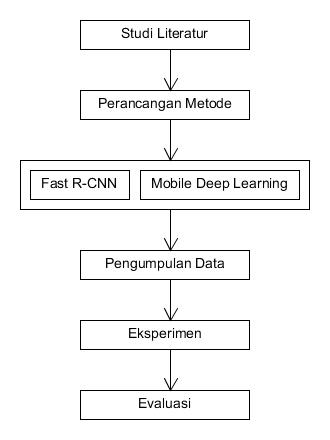
\includegraphics[width=8cm]{pics/metodologi_penelitian}
	\caption{Metodologi penelitian}
	\label{fig:metodologi_penelitian}
\end{figure}

Adapun penjelasan jenis kegiatan yang hendak dilaksanakan adalah sebagai
berikut:
\begin{enumerate}
	\item Studi literatur\\
	Pada tahap ini meliputi pengumpulan berbagai informasi tentang dasar teori serta penelitian-penelitian sebelumnya yang berkaitan dengan penelitian yang akan dilakukan. Tahapan ini bertujuan untuk mengetahui the state of the art dari penelitian yang berkaitan dengan pengenalan convolutional neural network dan deep learning pada teknologi mobile. Hasil kajian tersebut dijadikan sebagai acuan untuk mencari suatu pembaruan terhadap metode yang telah ada.
	\item Perancangan Metode\\
	Pada perancangan metode, ada 2 kegiatan umum yang akan dilakukan yaitu perancangan metode Fast R-CNN untuk melakukan deteksi batik dan metode Mobile Deep Learning untuk melakukan implementasi deep learning pada SoC mobile.
	\item Pengumpulan Data\\
	Pada penelitian menggunakan data batik yang berasal dari penelitian sebelumnya \cite{meta_cnn} dan terdiri dari 5 motif:
	\begin{itemize}
		\item Ceplok
		\item Kawung
		\item Lereng
		\item Nitik
		\item Parang
	\end{itemize}
	\item Eksperimen\\
	Eksperimen berdasarkan rancangan metode yang telah dibuat akan dilakukan menggunakan library Fast R-CNN pada https://github.com/rbgirshick/py-faster-rcnn dan NVIDIA Deep Neural Network library (cuDNN) untuk imeplemntasi pada platform mobile SoC.
	\item Evaluasi dan Analisis Hasil\\
	Pengujian hasil eksperimen meliputi pengujian performa dan akurasi. Selain itu, dalam penelitian ini juga akan dilakukan analisis terhadap waktu komputasi yang dibutuhkan oleh sistem dalam melakukan proses prapengolahan dokumen formulir, segmentasi tulisan dan pengenalan karakter.
\end{enumerate}

\section{Rencana Implementasi}
Secara umum, rencana eksperimen yang akan dilakukan dalam penelitian ini dapat dilihat pada \ref{fig:rencana_implementasi} berikut:
\begin{figure}[htp]
	\centering
	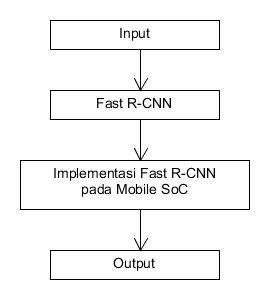
\includegraphics[width=8cm]{pics/rencana_implementasi}
	\caption{Rencana Implementasi}
	\label{fig:rencana_implementasi}
\end{figure}

Berdasarkan gambar \ref{fig:rencana_implementasi}, terdapat dua eksperimen utama yang akan dilakukan pada penelitian ini. Eksperimen pertama fokus kepada Fast R-CNN untuk pengenalan batik sedangkan pada eksperimen kedua fokus kepada implementasi Fast R-CNN pada perangkat mobile. Penjelasan untuk masing-masing proses adalah sebagai berikut:
\begin{enumerate}
	\item Tahap pertama\\
	Tahap pertama akan melakukan implementasi Fast R-CNN untuk mendeteksi batik sesuai dengan arsitektur pada gambar \ref{fig:arsitektur_fcnn}. Arsitektur Fast R-CNN \ref{fig:arsitektur_fcnn} memiliki input gambar secara keseluruhan dan kumpulan objek tertentu. Input akan diproses pertama kali kedalam beberapa layer konvolusi dan max pooling untuk mendapatkan feature map. Kemudian tiap objek proposal atau Region of Interest (RoI) akan melakukan ekstraksi fitur dari feature map. Tiap vektor fitur akan diproses secara berurutan kedalam Fully Connected Layer dan membagi ke dalam 2 output layer. Layer pertama menggunakan probabilitas softmax melakukan estimasi pada K kelas object dan kelas background. Layer kedua memberikan 4 output dalam bentuk bilangan real untuk tiap K kelas objek. Untuk setiap 4 nilai dilakukan encoding posisi bounding-box pada salah satu posisi dari kelas K.
	\item Tahap Kedua\\
	Tahap kedua akan berfokus pada implementasi Fast R-CNN pada perangkat mobile NVIDIA Tegra K-1 berdasarkan penelitian \cite{deepx}. Implementasi pada perangkat mobile akan mengoptimasi penggunaan sumber daya maupun waktu eksekusi dengan 2 pendekatan:
	\begin{enumerate}
		\item Runtime Layer Compression (RLC)\\
		RLC memeiliki 2 komponen utama, komponen pertama melakukan pengurangan dimensi untuk merendahkan kebutuhan komputasi tiap layer. komponen kedua berfungsi untuk mengatur level pengerungan dimensi yang akan diaplikasikan sebelum model akruasi dipengaruhi penggunan DeepX. Input kepada RLC adalah
		\begin{enumerate}
			\item sepasang adjacent layer dari model untuk dieksekusi
			\item Batas error yang digunakan oleh yang menggambarkan observasi dari rekonstruksi error setelah pengurangan dimensi dilakukan
		\end{enumerate}
		2 input tersebut disediakan oleh DAD yang juga menerima output dari RLS. secara spesifik, penggantian matiks bobot antara layer L dan L+1 yang membutuhkan parameter dan komputasi yang lebih sedikit.
		\item Deep Architecture Decomposition (DAD)\\
		DAD memeiliki 2 komponen diantaranya Decomposition Search dan Recomposition Inference. Komponen pertama bertujuan untuk memperhitungkan proses dekomposisi dari arsitektur deep secara efisien, kemudian dihitung performa estimasi sesuai dengan tujuan dari pengguna. RLS memperluas area pencarian DAD hingga kompresi layer dari beberapa rencana. komponen kedua melakukan inferensi hingga hasil model klasifikasi dengan melakukan rekomposisi hasil dekomposisi dari unitblock yang dialokasikan pada unit komputasi terpisah. input DAD terdiri dari:
		\begin{enumerate}
			\item model deep yang akan dieksekusi
			\item kumpulan tujuan performansi
		\end{enumerate}
		Output dari DAD adalah inferensi dari model input.		
	\end{enumerate}
\begin{figure}[htp]
	\centering
	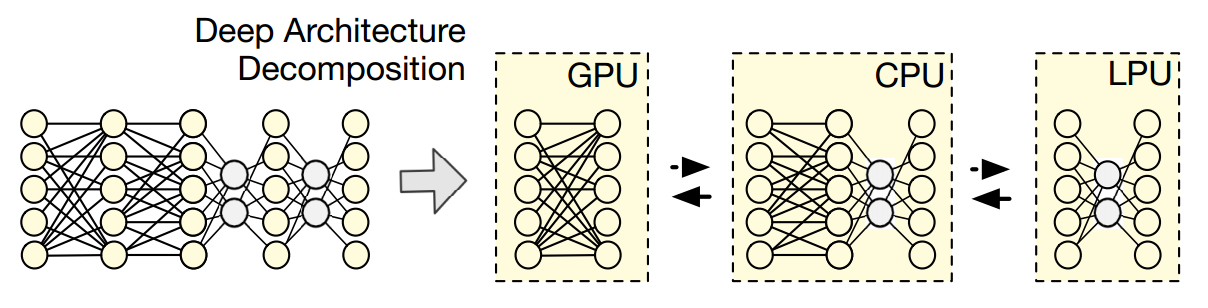
\includegraphics[width=10cm]{pics/dad}
	\caption{Deep Architecture Decomposition}
	\label{fig:dad}
\end{figure}
\end{enumerate}
\begin{figure}[htp]
	\centering
	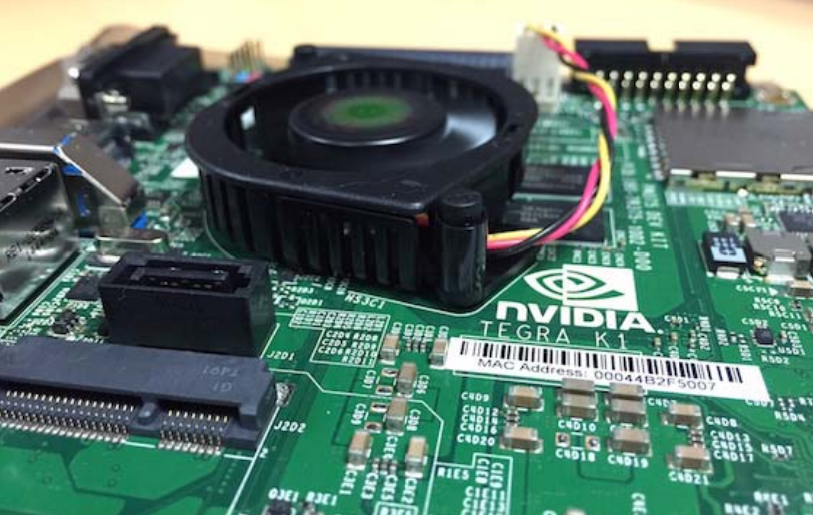
\includegraphics[width=8cm]{pics/tegra_k1}
	\caption{NVIDIA Tegra K1}
	\label{fig:tegra_k1}
\end{figure}